\documentclass[12pt]{article}
\usepackage{geometry}                % See geometry.pdf to learn the layout options. There are lots.
\geometry{letterpaper}                   % ... or a4paper or a5paper or ... 
%\geometry{landscape}                % Activate for for rotated page geometry
\usepackage[parfill]{parskip}    % Activate to begin paragraphs with an empty line rather than an indent
\usepackage{daves,fancyhdr,natbib,graphicx,dcolumn,amsmath,lastpage,url}
\usepackage{amsmath,amssymb,epstopdf,longtable}
\usepackage{paralist}  % need to modify standard enumerate blocks
\DeclareGraphicsRule{.tif}{png}{.png}{`convert #1 `dirname #1`/`basename #1 .tif`.png}
\pagestyle{fancy}
\lhead{CE 3354 -- Engineering Hydrology}
\rhead{SUMMER 2025}
\lfoot{EX3}
\cfoot{}
\rfoot{Page \thepage\ of \pageref{LastPage}}
\renewcommand\headrulewidth{0pt}



\begin{document}
\begin{center}
{\textbf{{ CE 3354 Engineering Hydrology} \\ {Exam 3}}}
\end{center}
\textbf{The actual examination was conducted using Canvas with auto-scoring.  This document is identical with regards to exam prompts}

\begin{enumerate}

\item (20 points) The map below is generated from the elevation survey indicated by the small points.  The weir outlet notch is at elevation 80, whereas the rest of the weir wall is at elevation 86.  The North edge of the map is a county road that drains North (forming a Northern boundary for the watershed).   

\begin{figure}[h!] %  figure placement: here, top, bottom, or page
   \centering
   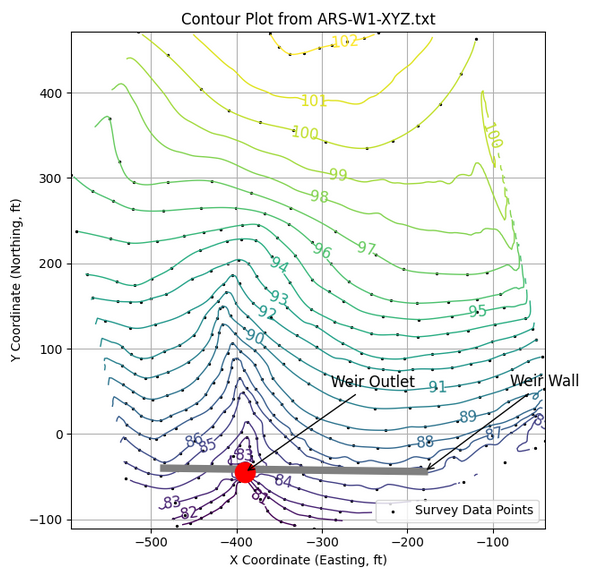
\includegraphics[width=5in]{ARS-W1_TopoMap.png} 
   \caption{Topographic map for ARS research watershed W-1 in Arkansas.}
   \label{fig:ARS-W1_TopoMap1}
\end{figure}

Delineate the boundary of the area that drains to the weir outlet on the map above.  Upload your delineated map as a PDF or PNG file.

\clearpage
%%%%%%%%%%%%%%%%%%%%%%%%%%%%%%%%%%%%%%%%%%%%%%%%%%%%%%%%%%%%
\item (10 points) The map below is generated from the elevation survey indicated by the small points.  The weir outlet notch is at elevation 80, whereas the rest of the weir wall is at elevation 86.  The North edge of the map is a county road that drains North (forming a Northern boundary for the watershed).   

\begin{figure}[h!] %  figure placement: here, top, bottom, or page
   \centering
   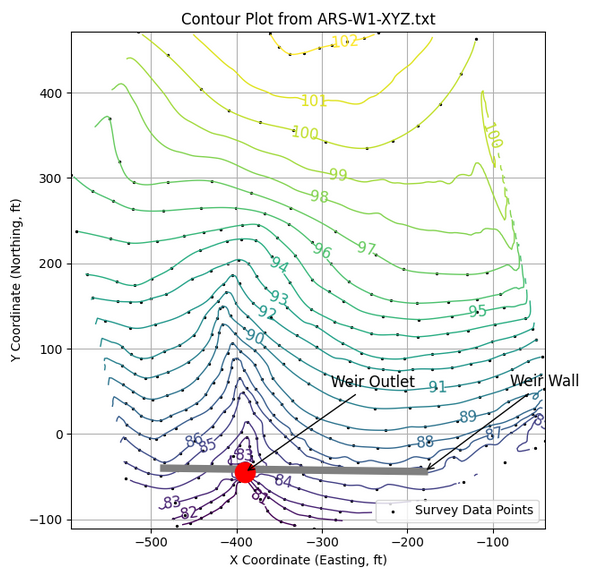
\includegraphics[width=5in]{ARS-W1_TopoMap.png} 
   \caption{Topographic map for ARS research watershed W-1 in Arkansas.}
   \label{fig:ARS-W1_TopoMap2}
\end{figure}

The drainage area of the watershed that drains to the weir outlet is closest to

    \begin{enumerate}[a)]
        \item 2.53 acres 
        \item 3.47 acres % answer
        \item 6.72 acres
        \item 7.57 acres
    \end{enumerate}

\clearpage
%%%%%%%%%%%%%%%%%%%%%%%%%%%%%%%%%%%%%%%%%%%%%%%%%%%%%%%%%%%%
\item (10 points) Heads (in feet) were measured in the 4 monitoring wells depicted on the figure below.  

\begin{figure}[h!] %  figure placement: here, top, bottom, or page
   \centering
   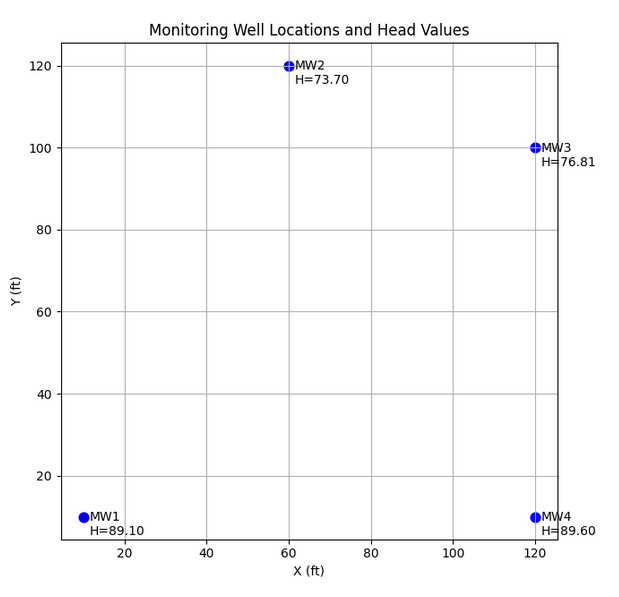
\includegraphics[width=5in]{MWplot.png} 
   \caption{Monitoring wells in an aquifer}
   \label{fig:MWP1}
\end{figure}

Using the data on the map the estimate for the magnitude of the hydraulic gradient in the region above is

    \begin{enumerate}[a)]
        \item 0.004
        \item 0.052
        \item 0.142 % answer
        \item 0.1663
    \end{enumerate}

\clearpage
%%%%%%%%%%%%%%%%%%%%%%%%%%%%%%%%%%%%%%%%%%%%%%%%%%%%%%%%%%%%
\item (10 points) Heads (in feet) were measured in the 4 monitoring wells depicted on the figure below.  

\begin{figure}[h!] %  figure placement: here, top, bottom, or page
   \centering
   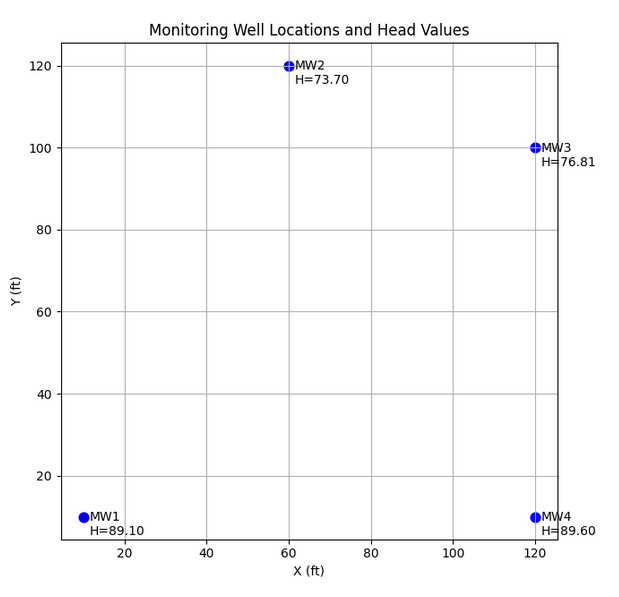
\includegraphics[width=5in]{MWplot.png} 
   \caption{Monitoring wells in an aquifer}
   \label{fig:MWP2}
\end{figure}

Using the data on the map the direction of groundwater flow in the region above is

    \begin{enumerate}[a)]
        \item North % answer
        \item South
        \item East
        \item West
    \end{enumerate}

\clearpage
%%%%%%%%%%%%%%%%%%%%%%%%%%%%%%%%%%%%%%%%%%%%%%%%%%%%%%%%%%%%%
\item (10 points) Heads (in feet) were measured in the 4 monitoring wells depicted on the figure below.  

\begin{figure}[h!] %  figure placement: here, top, bottom, or page
   \centering
   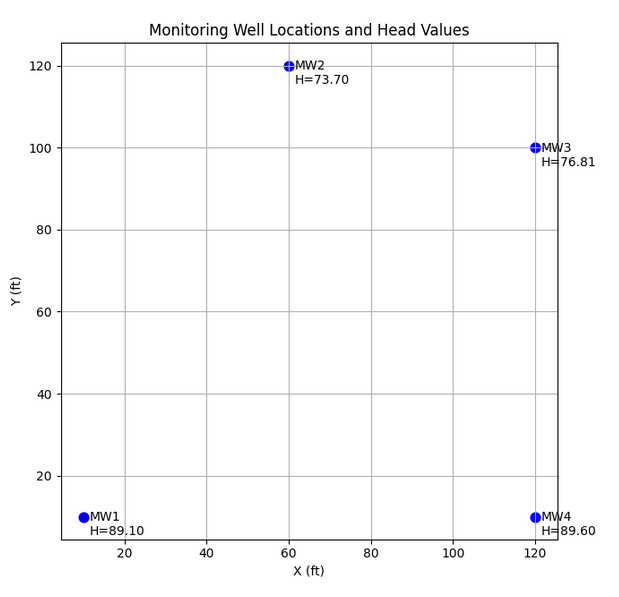
\includegraphics[width=5in]{MWplot.png} 
   \caption{Monitoring wells in an aquifer}
   \label{fig:MWP3}
\end{figure}

If the hydraulic conductivity is 10 feet/day, and the aquifer porosity is 0.30, the estimated travel time of a tracer particle released at (60,40) until it arrives at (60,120) is

    \begin{enumerate}[a)]
        \item 4.73 days
        \item 16.9 days % answer
        \item 56.3 days
        \item 266.7 days
    \end{enumerate}

\clearpage
%%%%%%%%%%%%%%%%%%%%%%%%%%%%%%%%%%%%%%%%%%%%%%%%%%%%%%%%%%%%%
\item (10 points) A well, PW1, in a confined aquifer is pumped at 3000 m3/day.  The transmissivity, T, is 1194 m2/day.  The storage coefficient, S, is 0.00012.   Three nearby wells in the aquifer are monitored from the start of pumping. MW1 is 150 meters from the pumping well, MW2 is 300 meters from the pumping well, and MW3 is 600 meters from the pumping well.

Using the Theis model determine the drawdown in three wells after 30 hours of pumping.

MW1 drawdown: [MW1] 
    \begin{enumerate}[a)]
        \item 0.90 meters
        \item 1.17 meters
        \item 1.44 meters % answer
        \item 2.30 meters
    \end{enumerate}

MW2 drawdown: [MW2] 
    \begin{enumerate}[a)]
        \item 0.90 meters
        \item 1.17 meters % answer
        \item 1.44 meters 
        \item 2.30 meters
    \end{enumerate}
MW3 drawdown: [MW3]
    \begin{enumerate}[a)]
        \item 0.90 meters % answer
        \item 1.17 meters 
        \item 1.44 meters 
        \item 2.30 meters
    \end{enumerate}
    
\clearpage
%%%%%%%%%%%%%%%%%%%%%%%%%%%%%%%%%%%%%%%%%%%%%%%%%%%%%%%%%%%%%
\item (10 points) During a drought period the following declines in the water table were recorded in an unconfined aquifer.

\begin{figure}[h!] %  figure placement: here, top, bottom, or page
   \centering
   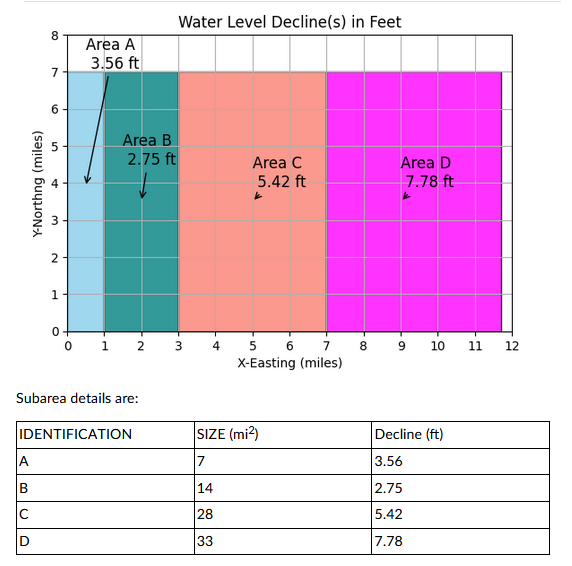
\includegraphics[width=6in]{Storage.png} 
   \caption{Plan view of aquifer region with avarage head declines by sub-area}
   \label{fig:Storage}
\end{figure}

The total volume of water removed from storage in this aquifer during the time period
was $5.7385 \times 10^4$ acre-feet.

An estimate of specific yield based on these data is

% 0.19 +/- 0.01  so 0.18-0.20 is anticipated result.
\clearpage
%%%%%%%%%%%%%%%%%%%%%%%%%%%%%%%%%%%%%%%%%%%%%%%%%%%%%%%%%%%%%
\item (20 points) The screen capture below is an attempt to compare computed combined hydrograph at the outlet for the May 27-29, 1975 storm on the watershed.   There is an error that needs repair.

\begin{figure}[h!] %  figure placement: here, top, bottom, or page
   \centering
   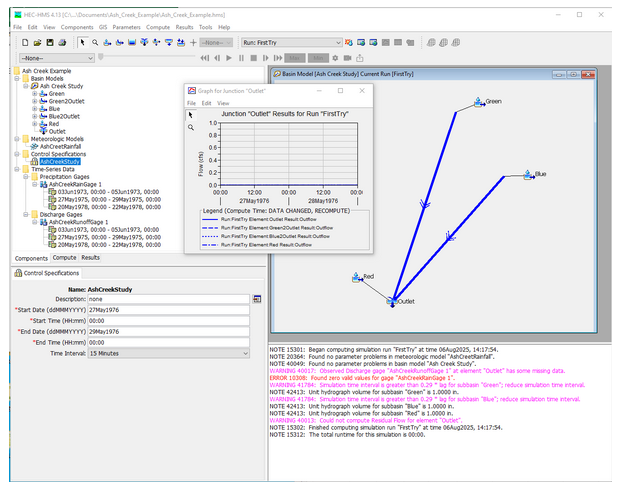
\includegraphics[width=6in]{HMS-Broke.png} 
   \caption{HEC-HMS screen capture; failed run}
   \label{fig:HMSBroke}
\end{figure}

Download the HMS project from AshCreekExample.zip\footnote{\url{http://54.243.252.9/ce-3354-webroot/hydrohandbook/exams/exam3/Ash_Creek_Example.zip}}.  You need to extract the .zip file (which is an entire HMS project).  Then open from HEC-HMS, make the repair and run the simulation.

Capture the output showing the computed total hydrograph and the observed hydrograph and upload a screen capture showing the result (i.e. a similar screen capture as above, but with the hydrographs showing).  Upload your result(s) as a PDF or PNG file.\footnote{On the Canvas/Moodle implementations these are uploaded to the server's MySQL database.  If administering live, students will need to print a screen capture to hand-in; or could send by email.}

\end{enumerate}



\end{document}  